
%% bare_conf.tex
%% V1.4b
%% 2015/08/26
%% by Michael Shell
%% See:
%% http://www.michaelshell.org/
%% for current contact information.
%%
%% This is a skeleton file demonstrating the use of IEEEtran.cls
%% (requires IEEEtran.cls version 1.8b or later) with an IEEE
%% conference paper.
%%
%% Support sites:
%% http://www.michaelshell.org/tex/ieeetran/
%% http://www.ctan.org/pkg/ieeetran
%% and
%% http://www.ieee.org/

%%*************************************************************************
%% Legal Notice:
%% This code is offered as-is without any warranty either expressed or
%% implied; without even the implied warranty of MERCHANTABILITY or
%% FITNESS FOR A PARTICULAR PURPOSE! 
%% User assumes all risk.
%% In no event shall the IEEE or any contributor to this code be liable for
%% any damages or losses, including, but not limited to, incidental,
%% consequential, or any other damages, resulting from the use or misuse
%% of any information contained here.
%%
%% All comments are the opinions of their respective authors and are not
%% necessarily endorsed by the IEEE.
%%
%% This work is distributed under the LaTeX Project Public License (LPPL)
%% ( http://www.latex-project.org/ ) version 1.3, and may be freely used,
%% distributed and modified. A copy of the LPPL, version 1.3, is included
%% in the base LaTeX documentation of all distributions of LaTeX released
%% 2003/12/01 or later.
%% Retain all contribution notices and credits.
%% ** Modified files should be clearly indicated as such, including  **
%% ** renaming them and changing author support contact information. **
%%*************************************************************************


% *** Authors should verify (and, if needed, correct) their LaTeX system  ***
% *** with the testflow diagnostic prior to trusting their LaTeX platform ***
% *** with production work. The IEEE's font choices and paper sizes can   ***
% *** trigger bugs that do not appear when using other class files.       ***                          ***
% The testflow support page is at:
% http://www.michaelshell.org/tex/testflow/



\documentclass[conference]{IEEEtran}
% Some Computer Society conferences also require the compsoc mode option,
% but others use the standard conference format.
%
% If IEEEtran.cls has not been installed into the LaTeX system files,
% manually specify the path to it like:
% \documentclass[conference]{../sty/IEEEtran}





% Some very useful LaTeX packages include:
% (uncomment the ones you want to load)


% *** MISC UTILITY PACKAGES ***
%
%\usepackage{ifpdf}
% Heiko Oberdiek's ifpdf.sty is very useful if you need conditional
% compilation based on whether the output is pdf or dvi.
% usage:
% \ifpdf
%   % pdf code
% \else
%   % dvi code
% \fi
% The latest version of ifpdf.sty can be obtained from:
% http://www.ctan.org/pkg/ifpdf
% Also, note that IEEEtran.cls V1.7 and later provides a builtin
% \ifCLASSINFOpdf conditional that works the same way.
% When switching from latex to pdflatex and vice-versa, the compiler may
% have to be run twice to clear warning/error messages.






% *** CITATION PACKAGES ***
%
\usepackage{cite}
% cite.sty was written by Donald Arseneau
% V1.6 and later of IEEEtran pre-defines the format of the cite.sty package
% \cite{} output to follow that of the IEEE. Loading the cite package will
% result in citation numbers being automatically sorted and properly
% "compressed/ranged". e.g., [1], \cite{rubinsztejn_framework_2005}, \cite{gamma_design_1995}, \cite{holder_system_1999}, \cite{pratikakis_transparent_2004}, \cite{_fusion_????} without using
% cite.sty will become [1], \cite{gamma_design_1995}, \cite{pratikakis_transparent_2004}--\cite{holder_system_1999}, \cite{rubinsztejn_framework_2005} using cite.sty. cite.sty's
% \cite will automatically add leading space, if needed. Use cite.sty's
% noadjust option (cite.sty V3.8 and later) if you want to turn this off
% such as if a citation ever needs to be enclosed in parenthesis.
% cite.sty is already installed on most LaTeX systems. Be sure and use
% version 5.0 (2009-03-20) and later if using hyperref.sty.
% The latest version can be obtained at:
% http://www.ctan.org/pkg/cite
% The documentation is contained in the cite.sty file itself.






% *** GRAPHICS RELATED PACKAGES ***
%
\ifCLASSINFOpdf
  \usepackage[pdftex]{graphicx}
  % declare the path(s) where your graphic files are
  % \graphicspath{{../pdf/}{../jpeg/}}
  % and their extensions so you won't have to specify these with
  % every instance of \includegraphics
  \DeclareGraphicsExtensions{.pdf,.jpeg,.png}
\else
  % or other class option (dvipsone, dvipdf, if not using dvips). graphicx
  % will default to the driver specified in the system graphics.cfg if no
  % driver is specified.
  \usepackage[dvips]{graphicx}
  % declare the path(s) where your graphic files are
  % \graphicspath{{../eps/}}
  % and their extensions so you won't have to specify these with
  % every instance of \includegraphics
  \DeclareGraphicsExtensions{.eps}
\fi
% graphicx was written by David Carlisle and Sebastian Rahtz. It is
% required if you want graphics, photos, etc. graphicx.sty is already
% installed on most LaTeX systems. The latest version and documentation
% can be obtained at: 
% http://www.ctan.org/pkg/graphicx
% Another good source of documentation is "Using Imported Graphics in
% LaTeX2e" by Keith Reckdahl which can be found at:
% http://www.ctan.org/pkg/epslatex
%
% latex, and pdflatex in dvi mode, support graphics in encapsulated
% postscript (.eps) format. pdflatex in pdf mode supports graphics
% in .pdf, .jpeg, .png and .mps (metapost) formats. Users should ensure
% that all non-photo figures use a vector format (.eps, .pdf, .mps) and
% not a bitmapped formats (.jpeg, .png). The IEEE frowns on bitmapped formats
% which can result in "jaggedy"/blurry rendering of lines and letters as
% well as large increases in file sizes.
%
% You can find documentation about the pdfTeX application at:
% http://www.tug.org/applications/pdftex





% *** MATH PACKAGES ***
%
\usepackage[fleqn]{amsmath}
% A popular package from the American Mathematical Society that provides
% many useful and powerful commands for dealing with mathematics.
%
% Note that the amsmath package sets \interdisplaylinepenalty to 10000
% thus preventing page breaks from occurring within multiline equations. Use:
%\interdisplaylinepenalty=2500
% after loading amsmath to restore such page breaks as IEEEtran.cls normally
% does. amsmath.sty is already installed on most LaTeX systems. The latest
% version and documentation can be obtained at:
% http://www.ctan.org/pkg/amsmath




% *** MATH PACKAGES ***
%
\usepackage{amssymb}





% *** SPECIALIZED LIST PACKAGES ***
%
\usepackage{algorithmic}
% algorithmic.sty was written by Peter Williams and Rogerio Brito.
% This package provides an algorithmic environment fo describing algorithms.
% You can use the algorithmic environment in-text or within a figure
% environment to provide for a floating algorithm. Do NOT use the algorithm
% floating environment provided by algorithm.sty (by the same authors) or
% algorithm2e.sty (by Christophe Fiorio) as the IEEE does not use dedicated
% algorithm float types and packages that provide these will not provide
% correct IEEE style captions. The latest version and documentation of
% algorithmic.sty can be obtained at:
% http://www.ctan.org/pkg/algorithms
% Also of interest may be the (relatively newer and more customizable)
% algorithmicx.sty package by Szasz Janos:
% http://www.ctan.org/pkg/algorithmicx




% *** ALIGNMENT PACKAGES ***
%
\usepackage{array}
% Frank Mittelbach's and David Carlisle's array.sty patches and improves
% the standard LaTeX2e array and tabular environments to provide better
% appearance and additional user controls. As the default LaTeX2e table
% generation code is lacking to the point of almost being broken with
% respect to the quality of the end results, all users are strongly
% advised to use an enhanced (at the very least that provided by array.sty)
% set of table tools. array.sty is already installed on most systems. The
% latest version and documentation can be obtained at:
% http://www.ctan.org/pkg/array


% IEEEtran contains the IEEEeqnarray family of commands that can be used to
% generate multiline equations as well as matrices, tables, etc., of high
% quality.




% *** SUBFIGURE PACKAGES ***
\ifCLASSOPTIONcompsoc
  \usepackage[caption=false,font=normalsize,labelfont=sf,textfont=sf]{subfig}
\else
  \usepackage[caption=false,font=footnotesize]{subfig}
\fi
% subfig.sty, written by Steven Douglas Cochran, is the modern replacement
% for subfigure.sty, the latter of which is no longer maintained and is
% incompatible with some LaTeX packages including fixltx2e. However,
% subfig.sty requires and automatically loads Axel Sommerfeldt's caption.sty
% which will override IEEEtran.cls' handling of captions and this will result
% in non-IEEE style figure/table captions. To prevent this problem, be sure
% and invoke subfig.sty's "caption=false" package option (available since
% subfig.sty version 1.3, 2005/06/28) as this is will preserve IEEEtran.cls
% handling of captions.
% Note that the Computer Society format requires a larger sans serif font
% than the serif footnote size font used in traditional IEEE formatting
% and thus the need to invoke different subfig.sty package options depending
% on whether compsoc mode has been enabled.
%
% The latest version and documentation of subfig.sty can be obtained at:
% http://www.ctan.org/pkg/subfig




% *** FLOAT PACKAGES ***
%
\usepackage{fixltx2e}
% fixltx2e, the successor to the earlier fix2col.sty, was written by
% Frank Mittelbach and David Carlisle. This package corrects a few problems
% in the LaTeX2e kernel, the most notable of which is that in current
% LaTeX2e releases, the ordering of single and double column floats is not
% guaranteed to be preserved. Thus, an unpatched LaTeX2e can allow a
% single column figure to be placed prior to an earlier double column
% figure.
% Be aware that LaTeX2e kernels dated 2015 and later have fixltx2e.sty's
% corrections already built into the system in which case a warning will
% be issued if an attempt is made to load fixltx2e.sty as it is no longer
% needed.
% The latest version and documentation can be found at:
% http://www.ctan.org/pkg/fixltx2e


\usepackage{stfloats}
% stfloats.sty was written by Sigitas Tolusis. This package gives LaTeX2e
% the ability to do double column floats at the bottom of the page as well
% as the top. (e.g., "\begin{figure*}[!b]" is not normally possible in
% LaTeX2e). It also provides a command:
%\fnbelowfloat
% to enable the placement of footnotes below bottom floats (the standard
% LaTeX2e kernel puts them above bottom floats). This is an invasive package
% which rewrites many portions of the LaTeX2e float routines. It may not work
% with other packages that modify the LaTeX2e float routines. The latest
% version and documentation can be obtained at:
% http://www.ctan.org/pkg/stfloats
% Do not use the stfloats baselinefloat ability as the IEEE does not allow
% \baselineskip to stretch. Authors submitting work to the IEEE should note
% that the IEEE rarely uses double column equations and that authors should try
% to avoid such use. Do not be tempted to use the cuted.sty or midfloat.sty
% packages (also by Sigitas Tolusis) as the IEEE does not format its papers in
% such ways.
% Do not attempt to use stfloats with fixltx2e as they are incompatible.
% Instead, use Morten Hogholm'a dblfloatfix which combines the features
% of both fixltx2e and stfloats:
%
% \usepackage{dblfloatfix}
% The latest version can be found at:
% http://www.ctan.org/pkg/dblfloatfix




% *** PDF, URL AND HYPERLINK PACKAGES ***
%
\usepackage{url}
% url.sty was written by Donald Arseneau. It provides better support for
% handling and breaking URLs. url.sty is already installed on most LaTeX
% systems. The latest version and documentation can be obtained at:
% http://www.ctan.org/pkg/url
% Basically, \url{my_url_here}.




%
%
\usepackage[bookmarks=false]{hyperref}
\newcommand{\algorithmautorefname}{Algorithm}




%
%
\usepackage{minted}
\usepackage{tcolorbox}
\usepackage{etoolbox}
\BeforeBeginEnvironment{minted}{\begin{tcolorbox}}%
\AfterEndEnvironment{minted}{\end{tcolorbox}}%
\AtBeginEnvironment{minted}{\fontsize{8}{8}}




%
% Digunakan untuk membuat inline list dan numbering
\usepackage{paralist}




%
% 
\usepackage{algorithm}
\usepackage{algorithmic}




%
% Digunakan untuk membuat tabel yang panjang, lebih dari 1 halaman
%
\usepackage{longtable, supertabular, booktabs}
  \newcommand{\ra}[1]{\renewcommand{\arraystretch}{#1}}




% *** Do not adjust lengths that control margins, column widths, etc. ***
% *** Do not use packages that alter fonts (such as pslatex).         ***
% There should be no need to do such things with IEEEtran.cls V1.6 and later.
% (Unless specifically asked to do so by the journal or conference you plan
% to submit to, of course. )


% correct bad hyphenation here
\hyphenation{op-tical net-works semi-conduc-tor}


\begin{document}
%
% paper title
% Titles are generally capitalized except for words such as a, an, and, as,
% at, but, by, for, in, nor, of, on, or, the, to and up, which are usually
% not capitalized unless they are the first or last word of the title.
% Linebreaks \\ can be used within to get better formatting as desired.
% Do not put math or special symbols in the title.
\title{An Architecture for Real-Time Location Recommendation for Field Data Collection}


% author names and affiliations
% use a multiple column layout for up to three different
% affiliations
\author{
\IEEEauthorblockN{Aris Prawisudatama}
\IEEEauthorblockA{School of Electrical Engineering and Informatics\\
Institut Teknologi Bandung\\
Bandung, Indonesia\\
Email: soedomoto@gmail.com}
\and
\IEEEauthorblockN{I Gusti Bagus Baskara Nugraha}
\IEEEauthorblockA{School of Electrical Engineering and Informatics\\
Institut Teknologi Bandung\\
Bandung, Indonesia\\
Email: baskara@stei.itb.ac.id}
}

% conference papers do not typically use \thanks and this command
% is locked out in conference mode. If really needed, such as for
% the acknowledgment of grants, issue a \IEEEoverridecommandlockouts
% after \documentclass

% for over three affiliations, or if they all won't fit within the width
% of the page, use this alternative format:
% 
%\author{\IEEEauthorblockN{Michael Shell\IEEEauthorrefmark{1},
%Homer Simpson\IEEEauthorrefmark{2},
%James Kirk\IEEEauthorrefmark{3}, 
%Montgomery Scott\IEEEauthorrefmark{3} and
%Eldon Tyrell\IEEEauthorrefmark{4}}
%\IEEEauthorblockA{\IEEEauthorrefmark{1}School of Electrical and Computer Engineering\\
%Georgia Institute of Technology,
%Atlanta, Georgia 30332--0250\\ Email: see http://www.michaelshell.org/contact.html}
%\IEEEauthorblockA{\IEEEauthorrefmark{2}Twentieth Century Fox, Springfield, USA\\
%Email: homer@thesimpsons.com}
%\IEEEauthorblockA{\IEEEauthorrefmark{3}Starfleet Academy, San Francisco, California 96678-2391\\
%Telephone: (800) 555--1212, Fax: (888) 555--1212}
%\IEEEauthorblockA{\IEEEauthorrefmark{4}Tyrell Inc., 123 Replicant Street, Los Angeles, California 90210--4321}}




% use for special paper notices
%\IEEEspecialpapernotice{(Invited Paper)}




% make the title area
\maketitle

% As a general rule, do not put math, special symbols or citations
% in the abstract
\begin{abstract}
Field data collection is one of the main activities performed by the national statistical agencies in every country. Data collection activities have a similar workflow with Multi-Depot Vehicle Routing Problem (MDVRP). The use of MDVRP to generate pre-calculated routes resulted in total route costs with high standard deviation. The real-time mechanism by utilizing the publish/subscribe paradigm combined with Cooperative Coevolution Algorithms (CoEAs) is proposed to reduce the inequality (large variation) of the completion time. The test results show that routes produced by the combination of publish/subscribe paradigm and CoEAs are more prevalent in total route times among enumerators compared with the pre-calculated routes produced by CoEAs only.
\end{abstract}

% no keywords




% For peer review papers, you can put extra information on the cover
% page as needed:
% \ifCLASSOPTIONpeerreview
% \begin{center} \bfseries EDICS Category: 3-BBND \end{center}
% \fi
%
% For peerreview papers, this IEEEtran command inserts a page break and
% creates the second title. It will be ignored for other modes.
\IEEEpeerreviewmaketitle




%-----------------------------------------------------------------------------%
\section{Introduction}
\label{sec:introduction}
%-----------------------------------------------------------------------------%
Data collection is one of the main duties of a statistical agency in every country. There are two data collection methods that are generally used: primary and secondary data collection. The primary data collection requires a direct interview with the respondents, while the secondary data collection only compiles the data collected by other agencies. Related to this, the primary data collection involves an activity of allocating the enumerators into several census/survey areas. The allocation is usually conducted by assigning an equal number of locations on each enumerator.

The workflow of the data collection performs as follows: 
\begin{enumerate}
	\item Each enumerator gets a list of census/survey locations to visit. 
	\item The enumeration starts on one particular point. It could be the statistical office or the enumerator's house. 
	\item The enumerator moves to the first census/survey location and visits all respondents in that location. 
	\item After finishing the first census/survey area, the enumerator moves to the second census/survey location and continue doing so until all locations have been visited successfully.
\end{enumerate}
This workflow is significantly similar to the Vehicle Routing Problem (VRP), specifically, the Multi-Depot Vehicle Routing Problem (MDVRP). The enumerators are analogous to vehicles, census/survey locations are comparable with customers, and the enumeration's starting point is corresponding with the depot. 

However, although sharing similar workflow with MDVRP, the rough implementation of the MDVRP algorithm is not feasible for solving the allocation problems. This is because MDVRP needs the variable \textit{service time}, which will not be available until after the enumerator finishes visiting the census/survey location. Therefore, this research aims to propose an integration of MDVRP with publish/subscribe mechanism to create a real-time location recommendation system for field data collection. 


%-----------------------------------------------------------------------------%
\section{Related Works}
\label{sec:related-works}
%-----------------------------------------------------------------------------%
%-----------------------------------------------------------------------------%
\subsection{Multi-Depot Vehicle Routing Problem (MDVRP)}
\label{ssec:mdvrp}
%-----------------------------------------------------------------------------%
VRP is an optimization problem that focused on the query: \textit{`given a set of vehicles and a starting point (depot), find the best route to visit all customers'}. In cases there is more than one depot, VRP is known as MDVRP \cite{montoya-torres_literature_2015}. \autoref{fig:mdvrp-illustration} shows an example of an MDVRP solution that uses two depots and two routes that associate with each depot. Basically, a solution for MDVRP is a set of routes such that: (i) each route starts and ends at the same depot, (ii) each customer is only served once by one vehicle, (iii) the total demand on each route does not exceed vehicle's capacity, (iv) the maximum route time is satisfied, and (v) the total cost is minimized.


\begin{figure}[!]
	\centering
	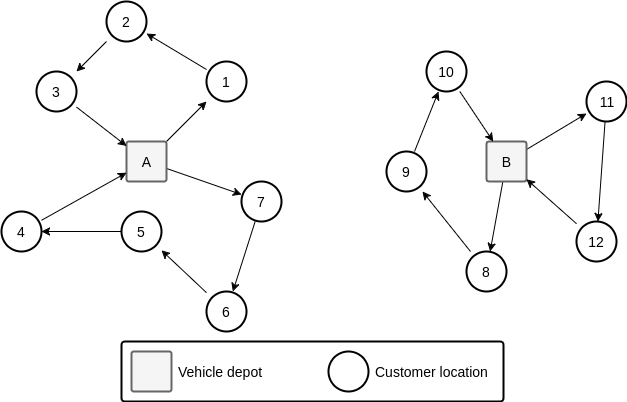
\includegraphics[width=8cm]{Resources/Images/mdvrp-illustration}
	\caption{An illustration for \textit{Multi Depot} VRP}
	\label{fig:mdvrp-illustration}
\end{figure}


According to Renaud et al \cite{renaud_tabu_1996}, the MDVRP can be formally described as follows:
\begin{enumerate}
	\item Let $G = (V, A)$ be a complete graph, where $V$ is the set of nodes and $A$ is the set of arcs. 
	\item Partition the nodes into two subsets: the customers to serve $V_C$ = \{1,..., $N$\} and the depots $V_D$ = \{$N$+1,..., $N+M$\}, with $V_C \cup V_D$ = $V$ and $V_C \cap V_D$ = $\oslash$. 
	\item There is a non-negative cost $c_{ij}$ associated with each arc $(i, j) \in A$. 
	\item The demand of each customer is $d_i$ (there is no demand at the depot nodes).
	\item There is also a fleet of $K$ identical vehicles, each with capacity $Q$.
	\item The service time at each customer $i$ is $t_i$ while the maximum route duration time is set to $T$.
	\item A conversion factor $w_{ij}$ might be needed to transform the cost $c_{ij}$ into time units. In the classical MDVRP, however, the cost is similar with the time and distance units. Hence, $w_{ij}$ = $1$.
\end{enumerate} 

In the math formula \cite{kulkarni_integer_1985}, binary variables $x_{ijk}$ are equal to $1$ when vehicle $k$ visits node $j$ immediately after node $i$. Auxiliary variable $y_i$ is also used in the subtour elimination constraints to indicate whether the route $i$ is used in the solution. \\


Minimize
\begin{flalign}
\label{eq:1}
\sum_{i=1}^{N+M}\sum_{j=1}^{N+M}\sum_{k=1}^{K}c_{ij}x_{ijk};
\end{flalign}


Subject to:
\begin{flalign}
\label{eq:2}
\sum_{i=1}^{N+M}\sum_{k=1}^{K}x_{ijk} = 1  (j=1,..., N);
\end{flalign}


\begin{flalign}
\label{eq:3}
\sum_{j=1}^{N+M}\sum_{k=1}^{K}x_{ijk} = 1  (j=1,..., N);
\end{flalign}


\begin{flalign}
\label{eq:4}
&\sum_{i=1}^{N+M}x_{ihk} - \sum_{j=1}^{N+M}x_{hjk} = 0 \\
\nonumber
&(k=1,...,K; h=1,...,N+M);
\end{flalign}


\begin{flalign}
\label{eq:5}
\sum_{i=1}^{N+M} \sum_{j=1}^{N+M} d_ix_{ijk} \leq Q (k=1,...,K);
\end{flalign}


\begin{flalign}
\label{eq:6}
\sum_{i=1}^{N+M} \sum_{j=1}^{N+M} (c_{ij}w_{ij} + t_i) x_{ijk} \leq T (k=1,...,K);
\end{flalign}


\begin{flalign}
\label{eq:7}
\sum_{i=N+1}^{N+M} \sum_{j=1}^{N} x_{ijk} \leq 1 (k=1,...,K);
\end{flalign}


\begin{flalign}
\label{eq:8}
\sum_{j=N+1}^{N+M} \sum_{i=1}^{N} x_{ijk} \leq 1 (k=1,...,K);
\end{flalign}


\begin{flalign}
\label{eq:9}
&y_i - y_j + (M + N)x_{ijk} \leq N + M - 1; \\
\nonumber
&for 1 \leq i \neq j \leq N and 1 \leq k \leq K;
\end{flalign}


\begin{flalign}
\label{eq:10}
x_{ijk} \in \{0, 1\} \forall i,j,k;
\end{flalign}


\begin{flalign}
\label{eq:11}
y_i \in \{0,1\} \forall i;
\end{flalign}


The objective \ref{eq:1} minimizes the total cost. Constraints \ref{eq:2} and \ref{eq:3} guarantee that each customer is served by exactly one vehicle. The flow conservation is guaranteed through constraint \ref{eq:4}. Vehicle capacity and route duration constraints are found in \ref{eq:5} and \ref{eq:6}, respectively. Constraints \ref{eq:7} and \ref{eq:8} check vehicle availability. Subtour elimination constraints are in \ref{eq:9}. Finally, \ref{eq:10} and \ref{eq:11} define x and y as binary variables.


%-----------------------------------------------------------------------------%
\subsection{Evolution Algorithms (EAs)}
\label{ssec:evolution-algorithms}
%-----------------------------------------------------------------------------%
Evolution Algorithms (EAs) is an optimization algorithm inspired by nature. EAs involve selection and reproduction processes to purify population from the solution candidates. According to Engelbrecht \cite{engelbrecht_coevolution_2007}, the EAs lifecycle begins with randomly configuring the initial population. For each iteration, every individual in the population is evaluated using an objective function to find the solution candidates. Each solution candidate is labeled with a fitness value based on its evaluation result. These candidates will then reproduce and create the next generation. The whole process will be repeated using the new-generation individuals. The iteration will stop once it hits a certain time limit, which is 60 seconds. 


In standard EAs, evolution is usually viewed as the population's attempts to adapt in a fixed physical environment. Furthermore, Coevolutionary algorithms (CoEAs), a development of EAs, realize that in natural evolution the physical environment is influenced by other independently-acting biological populations \cite{engelbrecht_coevolution_2007}. Based on the interaction of each species, CoEAs can be distinguished into two categories: competitive and cooperative \cite{engelbrecht_coevolution_2007}. In the competitive coevolution, each individual competes with other individuals in the same group. Meanwhile, the cooperative coevolution has its species mutually interacted or, at least, not harming each other. 


%-----------------------------------------------------------------------------%
\subsection{Publish/Subscribe Paradigm}
\label{ssec:pub-sub}
%-----------------------------------------------------------------------------%
The publish/subscribe interaction is a communication method between client and server, which involves subscribers as clients. The subscribers are the parties who have interests in a certain event or the pattern of an event. These subscribers will get a notification from the publisher about the event they are interested in \cite{eugster_many_2003}. 

The basic model of the publish/subscribe system, as can be seen in \autoref{fig:pub-sub-general}, depends on the event notification service that provides storage and management of subscription. This event service acts as a mediator between the publisher (the event's producer) and the subscriber (the event's consumer). 

\begin{figure}[!]
	\centering
	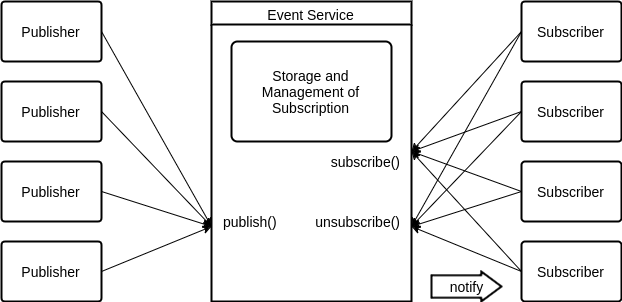
\includegraphics[width=8cm]{Resources/Images/pub-sub-general}
	\caption{Basic architecture in Publish/Subscribe Mechanism \cite{eugster_many_2003}}
	\label{fig:pub-sub-general}
\end{figure}


One of the benefits of using publish/subscribe mechanism is the loose coupling characteristic \cite{eugster_many_2003} between the publisher and the subscriber. The separation of information (decoupling) between publisher and subscriber can be divided into 3 (three) dimensions, which are:

\begin{enumerate}
	\item Space decoupling. \\
	During the interaction, publisher and subscriber do not need to know each other. The publisher sends an event and subscriber indirectly receives the event through the event service. The publisher does not hold any reference towards the subscriber and vice versa. 
	\item Time decoupling. \\
	The parties who are involved in the interactions do not have to interact in the same time. The publisher can send the event while in a disconnected state. Similarly, the subscriber can still receive the event, albeit disconnected. 
	\item Synchronizing decoupling. \\
	Publisher will not be blocked during the event producing. The subscriber can still obtain information despite, at the same time, working on other tasks. Publisher and subscriber are not in the main flow, hence not interacting synchronously. 
\end{enumerate}


%-----------------------------------------------------------------------------%
\section{Proposed Solution}
\label{sec:proposed-solution}
%-----------------------------------------------------------------------------%
The drawback of using MDVRP for location recommendation is the absence of time service data, which is very important for computing the recommendation. Thus, MDVRP needs to be integrated with a real-time mechanism such as Web Service, Remote Procedure Call (RPC), message passing, and publish/subscribe mechanism \cite{eugster_many_2003}.

In this research, the publish/subscribe mechanism is chosen because, in addition to its loose coupling characteristic, it is also suitable for an information-driven system \cite{muhl_large-scale_2002}. Loosing coupling allows the publish/subscribe mechanism to work asynchronously, meaning the request and the reply do not have to be processed in sequence. The publisher and subscriber can commit offline publishing and subscription, respectively. 


\begin{figure}[!]
	\centering
	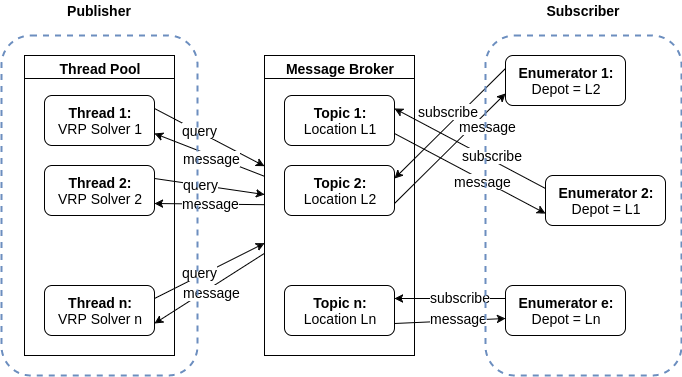
\includegraphics[width=8cm]{Resources/Images/system-overview}
	\caption{The outline of the proposed system}
	\label{fig:system-overview}
\end{figure}


\autoref{fig:system-overview} shows the system outline consists of 3 (three) main components: the publisher, the subscriber, and the message broker. The communication between publisher and subscriber is built upon their similarity in either event or topic. In this research, the subscriber's current location is chosen as the communication topic. 


%-----------------------------------------------------------------------------%
\subsection{The Recommendation Publisher}
\label{ssec:recommendation-publisher}
%-----------------------------------------------------------------------------%
VRP solver is implemented on the publisher's side. The publisher uses subscriber's current location as a topic to find the best solution/route. This route will be published to the subscriber via the message broker. The message broker plays a role in forwarding the message from publisher to subscriber and vice versa. Afterward, a new thread (\autoref{alg:topic-watcher}) is prepared to periodically check if there is any new topic at message broker. 

Every time a new topic emerges, a new thread will be created with that new topic used as an ID. Each thread contains VRP solver procedure (\autoref{alg:vrp-worker}) that acts as a solution/route finder. Accordingly, a thread pool is provided to accommodate all threads from each topic arranged in arrival order. Since the topic is used as a thread ID, the thread pool size is equal to the number of census/survey location. 


Each thread in the thread pool will be run consecutively, one session for each thread. Every running thread will find the solution by taking all $M$ vehicles and $(unassigned) N$ locations into account. This solution finding is performed using VRP solver procedure which is explained in more detail in \autoref{ssec:vrp-solver}.


\begin{algorithm}[!]
	\caption{TopicWatcher}
	\label{alg:topic-watcher}
	\begin{algorithmic}[1]
		\renewcommand{\algorithmicrequire}{\textbf{Input:}}
		\renewcommand{\algorithmicensure}{\textbf{Output:}}
		\REQUIRE $C$
		\ENSURE  $T$
		\FOR {$i = 1$ to $len(C)$}
			\FOR {$j = 1$ to $N$}
				\IF {($C_i == E_j$)}
					\STATE $T_j = Thread(C_i, V_1...V_M, (unassigned) E_1...E_N)$
				\ENDIF
			\ENDFOR
		\ENDFOR
		\RETURN $T$
	\end{algorithmic}
\end{algorithm}


The VRP solver procedure in each thread will produce at least $1$ route and at most $M$ routes. Every route $R_i$ that is produced will be published with a topic $C_i$. The message broker will inform the publisher the number of subscribers that receive the message. The subscribers' identities will remain unknown to the publisher. 


If a route $R_i$ has more than one message receiver, the thread with ID $C_{R_i}$ will be cancelled. This annulment is aimed to prevent a solution/route that has been received by subscribers from being recomputed. There could be a condition when the running VRP solver with ID $C_i$ does not produce the solution for topic $C_i$. In this situation, the topic $C_i$ will be requeued in thread pool by only involving the subscriber as the enumerator. As a result, there is a guarantee that every topic $C_i$ will have a solution/route. 


\begin{algorithm}[!]
	\caption{VRPWorker}
	\label{alg:vrp-worker}
	\begin{algorithmic}[1]
		\renewcommand{\algorithmicrequire}{\textbf{Input:}}
		\renewcommand{\algorithmicensure}{\textbf{Output:}}
		\REQUIRE $T$
		\ENSURE  $R$
		\FOR {$i = 1$ to $len(T)$}
			\STATE $R$ = VRPSolver($T_i$)
			\FOR {$j = 1$ to $len(R)$}
				\STATE $r$ = publish($C_{R_j}$, $R_j$)
				\IF {($r > 0$)}
					\STATE cancelSolver($T_j$)
				\ELSIF {($C_{T_i} \notin C_{R_j}$)}
					\STATE $T_i = Thread(C_{T_i}, V_m, (unassigned) E_1...E_N)$
				\ENDIF
			\ENDFOR
		\ENDFOR
		\RETURN $R$
	\end{algorithmic}
\end{algorithm}


Despite the flexibility, the loose coupling characteristics also brings a shortcoming to publish/subscribe mechanism. The publisher's unawareness towards subscribers' identities caused the subscribers' location cannot be identified. Hence, a mechanism that can support information exchange between publisher and subscribers is needed. The idea is to use a shared memory contains subscribers' current location data that can be accessed by the publisher. 

The whole processes described above, from detecting a new topic to obtaining the solution, will keep repeating until all customers are already assigned to each vehicle. In terms of data collection, the entire iterative processes will stop once all census/survey locations have been assigned to each enumerator. \autoref{fig:publisher-algorithm} illustrates the workflow of the algorithm used in recommendation publisher.


\begin{figure}[!]
	\centering
	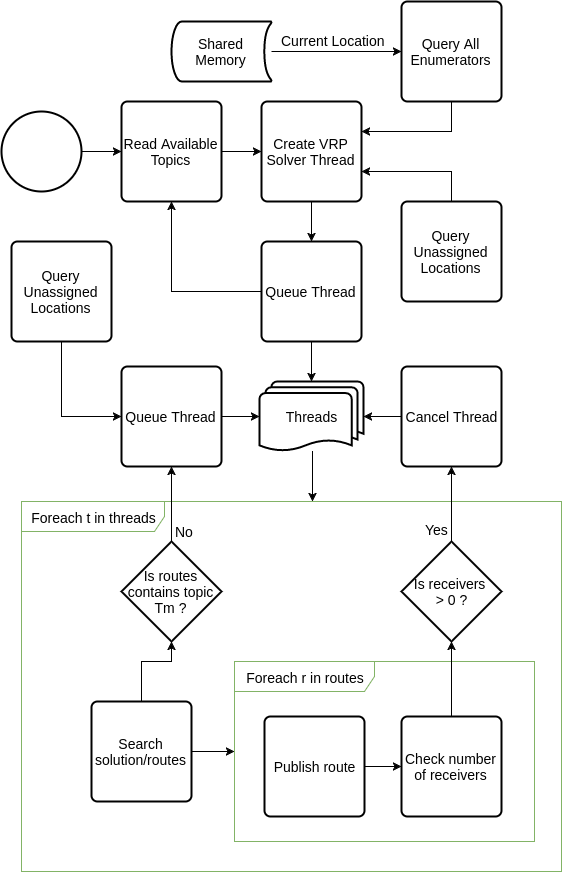
\includegraphics[width=8cm]{Resources/Images/publisher-algorithm}
	\caption{Publisher Workflow}
	\label{fig:publisher-algorithm}
\end{figure} 


%-----------------------------------------------------------------------------%
\subsection{VRP Solver}
\label{ssec:vrp-solver}
%-----------------------------------------------------------------------------%
VRP solver is a module used for finding the best route/solution to visit all customers (census/survey locations) in a VRP/MDVRP. VRP solver is called in each thread in the thread pool (\autoref{alg:vrp-worker}). There are several algorithms that can be adopted to find the solution such as tabu search \cite{cordeau_tabu_1997}, adaptive large neighborhood search  \cite{pisinger_general_2007}, fuzzy logic guided genetic algorithm \cite{lau_application_2010}, paralel iterated tabu search \cite{cordeau_parallel_2012}, hybrid algorithm combining iterated local search and set partitioning \cite{subramanian_hybrid_2013}, hybrid genetic algorithm with adaptive diversity control \cite{vidal_implicit_2014}, hybrid granular tabu search \cite{escobar_hybrid_2014}, and cooperative coevolution algorithms (CoEAs) \cite{de_oliveira_cooperative_2016}. In this research, VRP solver utilizes CoEAs since CoEAs generates a competitive \textit{mean solution values} with relatively low CPU time compared to other algorithms \cite{de_oliveira_cooperative_2016}. 


The VRP solver works as follows:
\begin{enumerate}
	\item Problem creation \\
	Create an instance of MDVRP that consists of $M$ vehicles (enumerators) and $N$ customers (locations).
	\item Problem decomposition \\
	Decompose the MDVRP into several subproblems using Nearest Insertion Heuristic (NIH) and Semi-greedy algorithm. Both of these algorithms are parts of CoEAs. 
	\item Individual evolution. \\
	Before each evolution, each individual in every subproblem is evaluated to find the current best individual (CBI) of all subproblems. Then, evolve each individual to generate new individuals. Evaluates these new individuals to find the new best individual (NBI). If NBI is better than CBI, update CBI with NBI value. Otherwise, leave the CBI as it is. Repeat the evolution process until it reaches the time limit of 60 seconds or 40 seconds if there is no change happens to the CBI.    
\end{enumerate}


\begin{algorithm}[!]
	\caption{VRPSolver}
	\label{alg:vrp-solver}
	\begin{algorithmic}[1]
		\renewcommand{\algorithmicrequire}{\textbf{Input:}}
		\renewcommand{\algorithmicensure}{\textbf{Output:}}
		\REQUIRE $T_i$
		\ENSURE  $R$
		\STATE P $\leftarrow$ createProblem($V_1...V_{T_i}$, $E_1...E_{T_i}$)
		\\ \textit{Decompose problem into S subproblem}
		\STATE SP $\leftarrow$ decomposeProblem(P)
		\WHILE {stopCriteriaUnmet}
			\FOR {$i=1$ to $len(SP)$}
				\STATE I $\leftarrow$ $SP_i \rightarrow individuals$
				\FOR {$j$ to $len(I)$}
					%\\ \textit{Foreach individu in subpopulation, do evolve}
					\STATE $O_j$ $\leftarrow$ $I_j \rightarrow evolve()$
				\ENDFOR
				\STATE shrink($I$, $O$)
			\ENDFOR
			%\\ \textit{Every iteration, update best individuals}
			\STATE updateBestIndividuals()
		\ENDWHILE
		\STATE $B \leftarrow getBestIndividuals()$ 
		\STATE $R \leftarrow convert(B)$ 
		\RETURN $R$
	\end{algorithmic}
\end{algorithm}


%-----------------------------------------------------------------------------%
\subsection{Message Broker}
\label{ssec:message-broker}
%-----------------------------------------------------------------------------%
A message broker is a component responsible for routing the message from publisher to subscriber based on the subscribed topic \cite{banavar_efficient_1999}. A publish/subscribe system can have a single broker or multi-broker. In single broker architecture, all subscribers and publishers are connected to one single broker, while in multi-broker architecture, every subscriber or publisher can connect to any nearest broker. This multi-broker architecture is also called distributed publish/subscribe system \cite{muhl_large-scale_2002} as depicted in \autoref{fig:pub_sub_distributed_ilustration}. In this research, the proposed design will implement distributed architecture since the census/survey locations are geographically scattered. 


\begin{figure}[!]
	\centering
	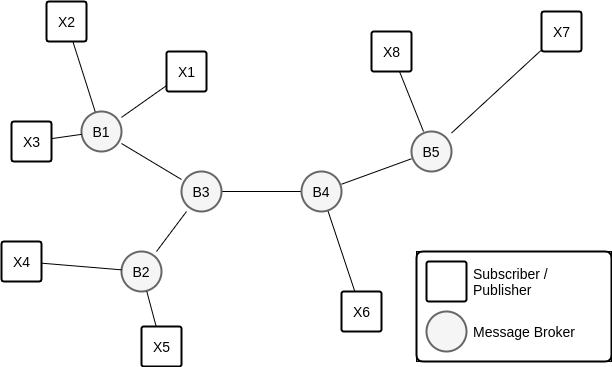
\includegraphics[width=7cm]{Resources/Images/pub_sub_distributed_ilustration}
	\caption{The architecture of distributed publish-subscribe}
	\label{fig:pub_sub_distributed_ilustration}
\end{figure}


%-----------------------------------------------------------------------------%
\section{Result}
\label{sec:testing}
%-----------------------------------------------------------------------------%
The performance of the proposed system is assessed through a number of experiments. This experiment uses 2 (two) input data: Cordeau's data and real administrative data. The service time for these two data is randomly generated by following the normal distribution. 


\begin{enumerate}
	\item The Cordeau's data \cite{cordeau_tabu_1997}, which consists of 50 customers (locations) and 4 vehicles (enumerators). The distances between locations are computed using euclidean formula. 
	\item The real administrative data, which consists of 182 customers (locations) and 15 vehicles (enumerators). The distances and the time needed to travel between locations are measured using Google Maps Direction API \cite{google_google_2016}. 
\end{enumerate}


These two data are tested using the proposed program, which combines Publish/Subscribe mechanism and CoEAs. The output of this test is compared against the output from the benchmark program that uses CoEAs algorithms only. Both programs output the routes for each vehicle which can be illustrated as follows:

\begin{itemize}
\item \textit{Vehicle} A = Loc1 $\rightarrow$ Loc5 $\rightarrow$ Loc15 $\rightarrow$ Loc6
\item \textit{Vehicle} B = Loc6 $\rightarrow$ Loc2 $\rightarrow$ Loc16 $\rightarrow$ Loc3
\item \textit{Vehicle} C = Loc4 $\rightarrow$ Loc8 $\rightarrow$ Loc14 $\rightarrow$ Loc 7
\item \textit{Vehicle} D = Loc9 $\rightarrow$ Loc10 $\rightarrow$ Loc11 $\rightarrow$ Loc12
\end{itemize}
where Loc is the location to visit. 

The total time for each route is calculated by adding up the service time and the transport time of all locations in that route. Standard deviation is used to compare the accuracy of output from proposed program and output from benchmark program. Standard deviation is chosen as the metric because it gives the insight about how diverse the output is, whether the outputs are close to the average or spread out over a wide range. The idea is the smaller variance of total time between each enumerator, the more equal and fairer the enumeration. Therefore, a better program will have smaller standard deviation.

The test using Cordeau's data in normal condition shows that the pre-calculated routes generated by benchmark program yield a smaller total time (1,165,513.28 seconds) compared with that of the proposed program (1,165,706.84 seconds). However, the benchmark program has, a bigger standard deviation of 98,268.51 seconds, in contrast with the proposed program of 12997.91 seconds (\autoref{tbl:test_result_normal_cordeau_comparison}). 

Similarly, the test using real administrative data in normal condition gives the result that pre-calculated routes from benchmark program return a smaller total time, yet a higher standard deviation compared with that of the proposed program. The benchmark program outputs a total time of 4,448,989.67 seconds and standard deviation of 119,720.84 seconds, while the proposed program gives total time of 4,559,658.67 seconds and standard deviation of 34,472.12 seconds (\autoref{tbl:test_result_normal_field_comparison}).


\begin{table}
	\centering
	\ra{1.3}
	\caption{The comparison between CoEAs algorithm and Pub/Sub + CoEAs algorithm for the Cordeau data}
	\label{tbl:test_result_normal_cordeau_comparison}
	\begin{tabular}{lrr}
		\toprule
			Units & CoEAs & CoEAs + Pub/Sub\\ 
		\midrule
			Total time (s) & 1165513.28 & 1165706.84\\
			Mean of time (s) & 291378.32 & 291426.71\\
			Std. Dev of time (s) & 98268.51 & 12997.91\\
		\bottomrule
	\end{tabular}
\end{table}


\begin{table}
	\centering
	\ra{1.3}
	\caption{The comparison between CoEAs algorithm and Pub/Sub + CoEAs algorithm for the real field data}
	\label{tbl:test_result_normal_field_comparison}
	\begin{tabular}{lrr}
		\toprule
			Units & CoEAs & CoEAs + Pub/Sub\\ 
		\midrule
			Total time (s) & 4448989.67 & 4559658.67\\
			Mean of time (s) & 296599.31 & 303977.24\\
			Std. Dev of time (s) & 119720.84 & 34472.12\\
		\bottomrule
	\end{tabular}
\end{table}


%-----------------------------------------------------------------------------%
\section{Conclusion and Future Works}
\label{sec:conclusion-future-works}
%-----------------------------------------------------------------------------%
This paper proposes the use of Cooperative Coevolutionary Algorithm (CoEAs) combined with Publish/Subscribe mechanism to solve the real-time location recommendation problem in field data collection. Based on the test results, it is concluded that: 

\begin{enumerate}
\item CoEAs algorithm outputs a more efficient route based on the total cost point of view, but, 
\item The CoEAs algorithm cannot be directly used in census/survey location recommendation since it contains a huge standard deviation of the total cost for each route, thus, 
\item The use of a real-time mechanism such as Publish/Subscribe mechanism is needed to overcome the inequality problem between each route. It means the tasks and locations will be more evenly distributed and every enumerator has equal workloads.
\end{enumerate}


Publish/Subscribe mechanism is not the only option that can be used to develop a real-time system. Further studies using other mechanisms such as Push/Pull mechanism and Request/Reply mechanism is required for comparison. A research on analyzing the performance of each mechanism in varying network conditions are also necessary to create a simulation of real field conditions.


% An example of a floating figure using the graphicx package.
% Note that \label must occur AFTER (or within) \caption.
% For figures, \caption should occur after the \includegraphics.
% Note that IEEEtran v1.7 and later has special internal code that
% is designed to preserve the operation of \label within \caption
% even when the captionsoff option is in effect. However, because
% of issues like this, it may be the safest practice to put all your
% \label just after \caption rather than within \caption{}.
%
% Reminder: the "draftcls" or "draftclsnofoot", not "draft", class
% option should be used if it is desired that the figures are to be
% displayed while in draft mode.
%
%\begin{figure}[!t]
%\centering
%\includegraphics[width=2.5in]{myfigure}
% where an .eps filename suffix will be assumed under latex, 
% and a .pdf suffix will be assumed for pdflatex; or what has been declared
% via \DeclareGraphicsExtensions.
%\caption{Simulation results for the network.}
%\label{fig_sim}
%\end{figure}

% Note that the IEEE typically puts floats only at the top, even when this
% results in a large percentage of a column being occupied by floats.


% An example of a double column floating figure using two subfigures.
% (The subfig.sty package must be loaded for this to work.)
% The subfigure \label commands are set within each subfloat command,
% and the \label for the overall figure must come after \caption.
% \hfil is used as a separator to get equal spacing.
% Watch out that the combined width of all the subfigures on a 
% line do not exceed the text width or a line break will occur.
%
%\begin{figure*}[!t]
%\centering
%\subfloat[Case I]{\includegraphics[width=2.5in]{box}%
%\label{fig_first_case}}
%\hfil
%\subfloat[Case II]{\includegraphics[width=2.5in]{box}%
%\label{fig_second_case}}
%\caption{Simulation results for the network.}
%\label{fig_sim}
%\end{figure*}
%
% Note that often IEEE papers with subfigures do not employ subfigure
% captions (using the optional argument to \subfloat[]), but instead will
% reference/describe all of them (a), (b), etc., within the main caption.
% Be aware that for subfig.sty to generate the (a), (b), etc., subfigure
% labels, the optional argument to \subfloat must be present. If a
% subcaption is not desired, just leave its contents blank,
% e.g., \subfloat[].


% An example of a floating table. Note that, for IEEE style tables, the
% \caption command should come BEFORE the table and, given that table
% captions serve much like titles, are usually capitalized except for words
% such as a, an, and, as, at, but, by, for, in, nor, of, on, or, the, to
% and up, which are usually not capitalized unless they are the first or
% last word of the caption. Table text will default to \footnotesize as
% the IEEE normally uses this smaller font for tables.
% The \label must come after \caption as always.
%
%\begin{table}[!t]
%% increase table row spacing, adjust to taste
%\renewcommand{\arraystretch}{1.3}
% if using array.sty, it might be a good idea to tweak the value of
% \extrarowheight as needed to properly center the text within the cells
%\caption{An Example of a Table}
%\label{table_example}
%\centering
%% Some packages, such as MDW tools, offer better commands for making tables
%% than the plain LaTeX2e tabular which is used here.
%\begin{tabular}{|c||c|}
%\hline
%One & Two\\
%\hline
%Three & Four\\
%\hline
%\end{tabular}
%\end{table}


% Note that the IEEE does not put floats in the very first column
% - or typically anywhere on the first page for that matter. Also,
% in-text middle ("here") positioning is typically not used, but it
% is allowed and encouraged for Computer Society conferences (but
% not Computer Society journals). Most IEEE journals/conferences use
% top floats exclusively. 
% Note that, LaTeX2e, unlike IEEE journals/conferences, places
% footnotes above bottom floats. This can be corrected via the
% \fnbelowfloat command of the stfloats package.


% conference papers do not normally have an appendix


% use section* for acknowledgment
% \section*{Acknowledgment}
% The authors would like to thank...





% trigger a \newpage just before the given reference
% number - used to balance the columns on the last page
% adjust value as needed - may need to be readjusted if
% the document is modified later
%\IEEEtriggeratref{8}
% The "triggered" command can be changed if desired:
%\IEEEtriggercmd{\enlargethispage{-5in}}

% references section

% can use a bibliography generated by BibTeX as a .bbl file
% BibTeX documentation can be easily obtained at:
% http://mirror.ctan.org/biblio/bibtex/contrib/doc/
% The IEEEtran BibTeX style support page is at:
% http://www.michaelshell.org/tex/ieeetran/bibtex/
% bibliographystyle{IEEEtran}
% argument is your BibTeX string definitions and bibliography database(s)
% bibliography{IEEEabrv,Paper.bib}
%
% <OR> manually copy in the resultant .bbl file
% set second argument of \begin to the number of references
% (used to reserve space for the reference number labels box)
% \begin{thebibliography}{1}

% \bibitem{IEEEhowto:kopka}
% H.~Kopka and P.~W. Daly, \emph{A Guide to \LaTeX}, 3rd~ed.\hskip 1em plus
%   0.5em minus 0.4em\relax Harlow, England: Addison-Wesley, 1999.

% \end{thebibliography}

\bibliographystyle{IEEEtran}
\bibliography{Resources/Bib/Reference}


% that's all folks
\end{document}


